\documentclass{article}


\usepackage{PRIMEarxiv}

\usepackage[utf8]{inputenc} % allow utf-8 input
\usepackage[T1]{fontenc}    % use 8-bit T1 fonts
\usepackage{hyperref}       % hyperlinks
\usepackage{url}            % simple URL typesetting
\usepackage{booktabs}       % professional-quality tables
\usepackage{amsfonts}       % blackboard math symbols
\usepackage{nicefrac}       % compact symbols for 1/2, etc.
\usepackage{microtype}      % microtypography
\usepackage{lipsum}
\usepackage{fancyhdr}       % header
\usepackage{graphicx}       % graphics
\graphicspath{{media/}}     % organize your images and other figures under media/ folder

%Header
\pagestyle{fancy}
\thispagestyle{empty}
\rhead{ \textit{ }} 

% Update your Headers here
\fancyhead[LO]{Video Diffusion for Sign Language Translation}
% \fancyhead[RE]{Firstauthor and Secondauthor} % Firstauthor et al. if more than 2 - must use \documentclass[twoside]{article}



  
%% Title
\title{Video Diffusion for Sign Language Translation
%%%% Cite as
%%%% Update your official citation here when published 
\thanks{\textit{\underline{Code}}: 
\url{https://github.com/jaded0/sign-translation/tree/vid-signs}} 
}

\author{
  Jaden Lorenc \\
  student \\
  BYU \\
  Provo, Utah\\
  jaden.lorenc@gmail.com
  \And 
  Brooklyn Lorenc \\
  student \\
  BYU \\
  Provo, Utah\\
  brooklynbrightonk@gmail.com
}

\begin{document}
\maketitle


\begin{abstract}
This paper explores the use of video diffusion models for sign language translation from signed to written language. The limited availability of sign language data presents a low-resource problem, with the largest dataset containing only a word-level collection of 12,000 videos representing 2,000 unique signs in American Sign Language. The author investigates the temporal representation of signs through existing video diffusion techniques and secondary details such as race, accent, and surroundings using fine-tuning of larger diffusion models for images. They ran experiments with different hyperparameters, batch sizes, frame counts, and temporal downsampling factors. They also explored using publicly available Stable Diffusion weights for fine-tuning the model, which could potentially address issues of racial and gender bias. The author plans to conduct more structured experiments on the effects of parameters on the 16px model and believes that the resulting model could allow for the training of higher resolution models.
\end{abstract}


% keywords can be removed
\keywords{First keyword \and Second keyword \and More keywords}


\section{Introduction}
While sign language translation research appears to focus on the translation from signed to written language, comparatively little research attempts to do the reverse. The translation from signed to written language is also a low-resource problem, with the largest dataset available in American Sign Language being only a word-level collection of about twelve thousand videos representing two thousand unique signs. Given the success of recent diffuser based text-to-image generation models, it's possible that video diffusion may address the scarcity of data in sign translations contexts. In this report, I explore, separately, two attributes of such a model. The first is temporal representation of the sign, implemented via existing video diffusion techniques. The second is secondary details, such as the race of the signer, their signing accent, or their physical surroundings. This is implemented via fine-tuning of larger diffusion models for images.

\section{Video Diffusion}
The primary barrier here seems to be computational resources. Using, as a starting point, code based on Video Diffusion Models \cite{videodiffusion} found here,
\url{https://github.com/lucidrains/imagen-pytorch} I initially attempted to use a cascading model on prohibitively high image sizes and unet dimensions. Runs were slow. The smaller model created an acceptable result within three days, but the larger one, initially trained for 64 pixels was run for several months with various tweaks but showed slow progress \ref{fig:fig1}. Other initial choices include cascading diffusion and minor random image cropping. 
\begin{figure}
  \centering
  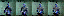
\includegraphics[scale=5]{book.png}
  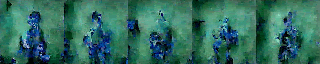
\includegraphics[scale=1]{bigbook.png}
  \caption{Some frames from the 16x16 pixel and 64x64 pixel animations for the sign, 'book.'}
  \label{fig:fig1}
\end{figure}

Some validation with the final 16-pixel videos was promising; when given a video and four possible words, a signer was able to identify the corresponding word the majority of the time. However, the larger, 64-pixel model never created identifiable signs. 

\subsection{Larger Resources}
I gained access to Nvidia A100 GPUs, opening up more options as far as batch size and model size. I ran once for nine hours, and in an attempt to speed up training, I explored many different hyperparameter configurations. I first used as large a batch size as possible, but noticed that the runs were slower. I noticed a sharp drop in loss numbers as I pulled the frame count of the sampled videos down to four, so I ran further experiments with progressively smaller batch sizes and slightly higher numbers of video frames \ref{fig:fig2}. A larger batch size clearly increased the loss variance, but didn't change the speed of the training. GPU usage and memory metrics support the idea that more usage occurs with the smaller batch sizes and frame counts, and  However, each trial ran from the checkpoints of the last, sacrificing conclusivity for the hope of a more impressive end result. 

\begin{figure}
  \centering
  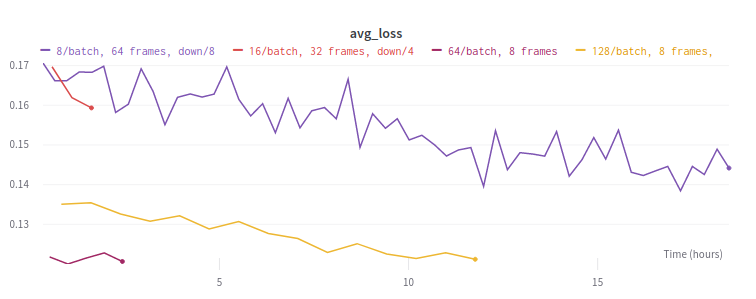
\includegraphics[scale=0.5]{graph.png}
  \caption{Loss numbers from a scattered exploration of batch size, frame count, and temporal downscaling factor.}
  \label{fig:fig2}
\end{figure}

Additionally, I began to experiment with temporal downsampling, after having learned about modern self-supervised strategies used in other tasks. I imagined that, as other models gained accuracy by invariance to features such as color, my model might benefit in training speed by being time-invariant, while also benefitting from faster training time by eliminating frames. The distance between frames chosen from the sample does not vary at training time, though, so the former conclusion remains to be seen. Temporal downsampling does, however, allow me to speed up the model's training by reducing the number of frame which need to be processed. The most recent videos generated by the model can be seen at \url{https://wandb.ai/jadens_team/vid-signs/runs/8weja1ku?workspace=user-jaden-lorenc}

\subsection{Next Steps}
I will perform a more structured experiment on the effects of batch size, frame count, and temporal downsampling factor on the the 16px model. The hope is that I'll find a balance of parameters that more quickly trains the higher resolutions. 

\section{Fine-Tuned Image Diffusion}
An advantage to creating a back-translation using image generating models is that features not present in the limited sign language dataset can be gained from other images or in the weights of large pretrained diffusion models. The goal with using the publicly available Stable Diffusion weights is to more quickly train my own model, while also retaining representations not found in the WLASL dataset. 

\subsection{Racial and Gender Bias Correction}
An excellent example is that of racial and gender bias, an issue that is already identified and worked on in existing papers on sign language translation \cite{8650524}. On the new fine-tuned model, the signer's race can be selected in the prompt\ref{fig:fig3}. Given a sufficiently diverse initial model, the resulting translation model can possibly become unbiased.
\begin{figure}
  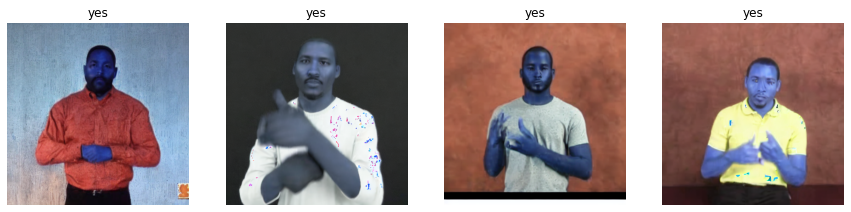
\includegraphics[scale=0.5]{black_yes.png}
  \caption{Prompt: "a black man signing, sign language for: yes"}
  \label{fig:fig3}
  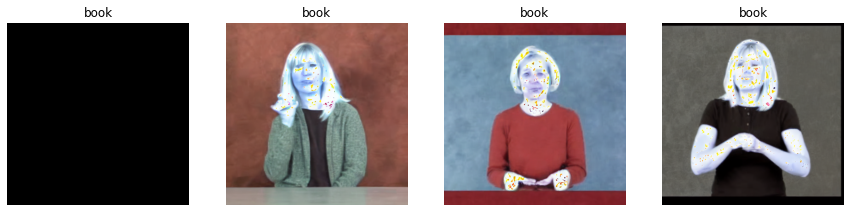
\includegraphics[scale=0.5]{lady_book.png}
  \caption{Prompt: "sign language for: book"}
  \label{fig:fig4}
\end{figure}

\subsection{Sign Accuracy}
Similar signs are classified in terms of shared hand shape, palm orientation, hand location, movement, whether they're one-handed or two-handed signs, and facial expressions. American Sign Language is considered a high-context language, but WLASL is only a word-level dataset. All of the sample words are removed from context, resulting in many typically co-occuring parameters not being expressed in the model's training set and therefore its outputs. However, most of the resulting samples still fail to fall semantically close to the label. The third sample shown for 'book' is exceptional for only failing in terms palm orientation. 
I attribute the low sign accuracy to a short training time, but longer training time leads to artifacts which impair other aspects of the results. Catastrophic forgetting is the likely culprit, so further investigation into its prevention will be the key to allowing for more training time, and thus, emphasis on sign accuracy. 

\section{Conclusion}
Validation has been gathered on the feasibility of diffusion models' ability to both bring in features from outside a given signed dataset and, separately, begin to represent animated signs with rough identifiability. Further investigation will entail more efficient video diffusion training on higher resolutions, explorations in time invariance, and the integration and preservation of pretrained weights into the video diffusion model. 

%Bibliography
\bibliographystyle{unsrt}  
\bibliography{references}  


\end{document}
